\documentclass[12pt]{extarticle}
\usepackage[english,ukrainian]{babel}
\usepackage[utf8]{inputenc}
\usepackage{amsmath,amssymb}
\usepackage{parskip}
\usepackage{graphicx}
\usepackage{xcolor}
\usepackage{tcolorbox}
\tcbuselibrary{skins}
\usepackage[framemethod=tikz]{mdframed}
\usepackage{chngcntr}
\usepackage{enumitem}
\usepackage{hyperref}
\usepackage{float}
\usepackage{subfig}
\usepackage{esint}
\usepackage[top=2.5cm, left=3cm, right=3cm, bottom=4.0cm]{geometry}
\usepackage[table]{xcolor}
\usepackage{algorithm}
\usepackage{algpseudocode}
\usepackage{listings}

\title{Індивідуальне завдання з курсу ``Теоретична механіка''}
\author{Студента 3 курсу групи МП-31 Захарова Дмитра}
\date{\today}

\begin{document}

\maketitle

\textbf{Варіант 18}
\section*{Завдання} Точка $M$ рухається відносно тіла. За заданими рівняннями відносного руху точки $M$ та руху тіла визначити для моменту часу $t=t_1$ абсолютну швидкість та прискорення $M$.
\[
OM(t) =: s(t) = 10t+t^3 \, (\text{cm}),\;\varphi(t)=8t-t^2\, (\text{rad}),\;t_1=2 \, \text{s}, \; \alpha=\frac{\pi}{3}
\]

\begin{figure}[H]
    \centering
    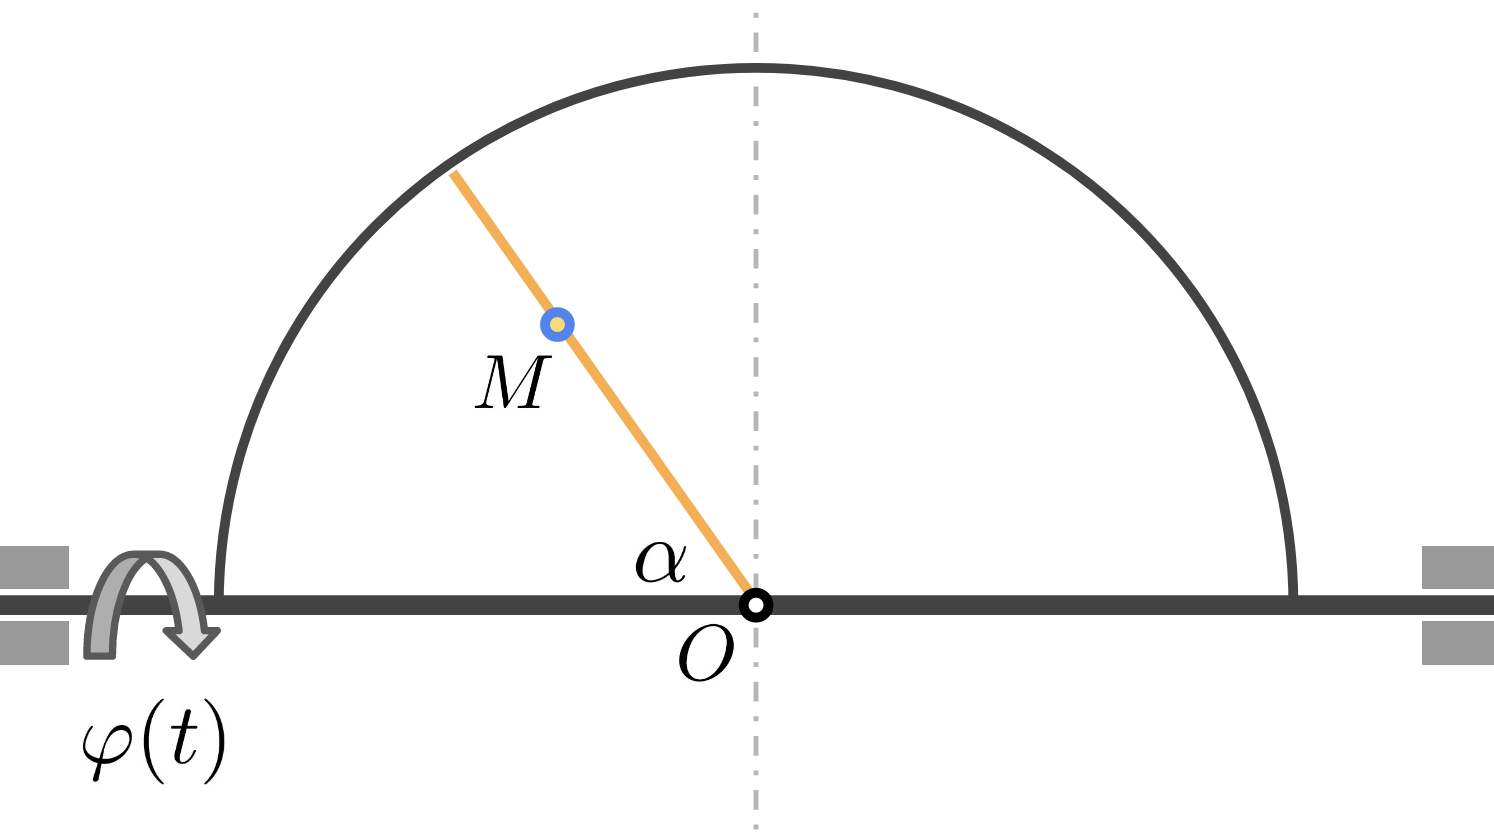
\includegraphics[width=0.8\textwidth]{images/test_1/fig_1.png}
    \caption{Умова завдання}
    \label{fig:1}
\end{figure}

\pagebreak
\section*{Розв'язок.}

\textbf{Спосіб I.} Виведемо конкретну функцію радіус-вектору точки $M$ від часу, а по ній легко знайдемо швидкість та прискорення.

Введемо систему координат, як показано на рисунку \ref{fig:2} (вісь $Oz$ дивиться на нас).

\begin{figure}[H]
    \centering
    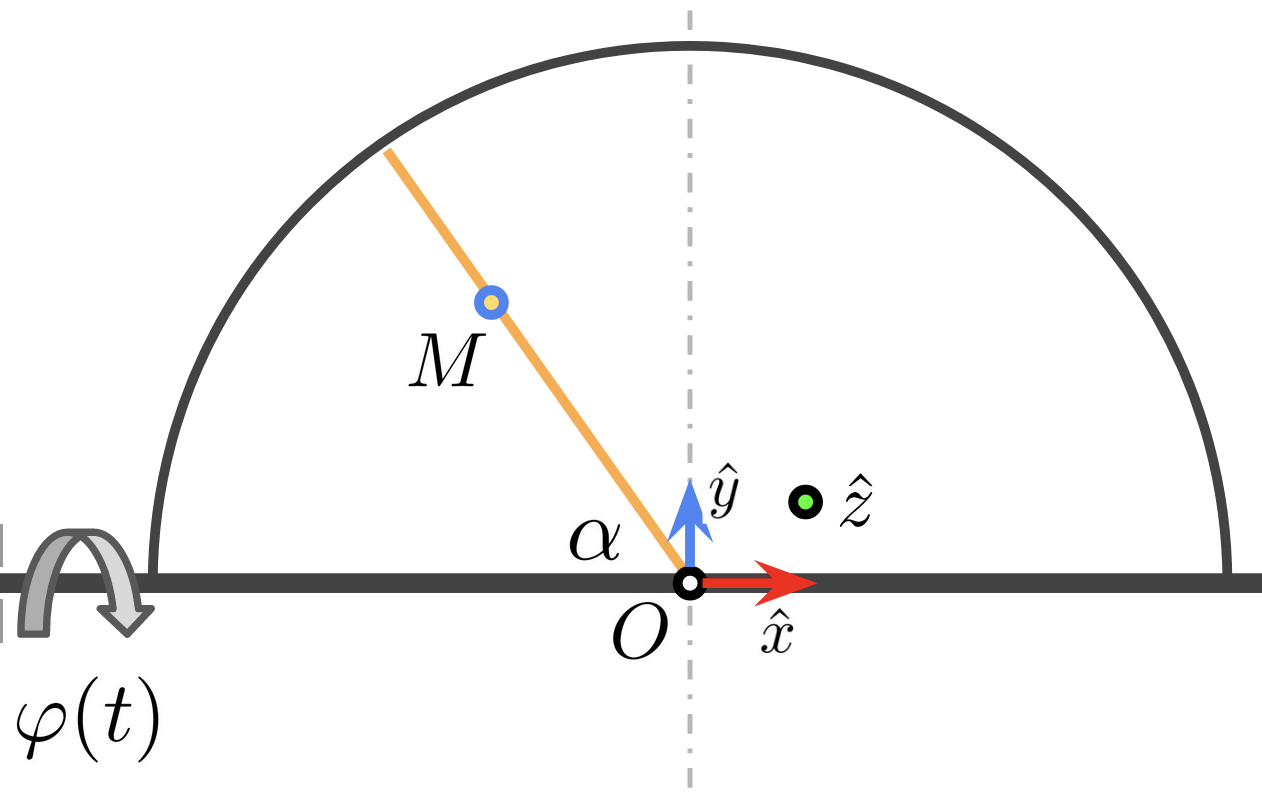
\includegraphics[width=0.5\textwidth]{images/test_1/fig_2.png}
    \caption{Введення системи координат}
    \label{fig:2}
\end{figure}

У відносній системі координат тіла (тобто якщо прийняти, що базиси $\hat{x}$ та $\hat{y}$ рузаються разом з тілом; позначимо такий базис як $\hat{x}',\hat{y}'$), точка має координати 
\[
\widetilde{\mathbf{r}}_M(t) = -s(t)\cos \alpha \hat{x}' + s(t)\sin \alpha \hat{y}'
\]
Проте, нас цікавлять саме абсолютні координати. Для цього помітимо, що нам потрібно повернути $M$ на кут $\varphi(t)$ навколо вісі $Ox$. Для цього, достатньо помножити вектор $\mathbf{r}_M(t)$ на матрицю повороту
\[
\boldsymbol{R}_{Ox}(\varphi) = \begin{bmatrix}
    1 & 0 & 0 \\ 0 & \cos \varphi & -\sin \varphi \\ 0 & \sin \varphi & \cos \varphi
\end{bmatrix}
\]
Отже:
\[
\mathbf{r}_M(t) = \begin{bmatrix}
    1 & 0 & 0 \\ 0 & \cos \varphi & -\sin \varphi \\ 0 & \sin \varphi & \cos \varphi
\end{bmatrix}\begin{bmatrix}
    -s \cos \alpha \\ s \sin \alpha \\ 0
\end{bmatrix} = \begin{bmatrix}
    -s \cos \alpha \\ s \sin \alpha \cos \varphi \\ s \sin \alpha \sin \varphi
\end{bmatrix}
\]
Таким чином,
\[
\mathbf{v}_M = \dot{\mathbf{r}}_M = -\dot{s} \cos\alpha \hat{x} + (\dot{s}\cos\varphi - s\dot{\varphi}\sin\varphi)\sin\alpha\hat{y} + (\dot{s}\sin\varphi + s\dot{\varphi}\cos\varphi)\sin\alpha\hat{z}
\]
Таким чином, модуль:
\[
v_M^2 = \dot{s}^2\cos^2\alpha + (\dot{s}^2+s^2\dot{\varphi}^2)\sin^2\alpha = \dot{s}^2 + s^2\dot{\varphi}^2 \sin^2\alpha
\]
Підставимо числа. $\dot{s}=10+3t^2,\dot{\varphi}=8-2t$, тому $s(t_1)=28,\dot{s}(t_1)=22$. Окрім цього, $\varphi(t_1)=12,\;\dot{\varphi}(t_1)=4$. Тому:
\[
v_M^2(t_1) = \left(22^2 + 28^2 \cdot 4^2 \cdot \frac{3}{4}\right) \, \frac{\text{cm}^2}{\text{s}^2} \implies v_M \approx 99.46 \, \text{cm/s} \approx 9.95 \, \text{m}/\text{s}
\]
Тепер знайдемо похідну ще раз, запишемо все покомпонентно:
\[
(a_M)_x = -\ddot{s} \cos \alpha 
\]
\[
(a_M)_y = (\ddot{s}\cos\varphi - 2\dot{s}\dot{\varphi}\sin\varphi - s\ddot{\varphi}\sin\varphi - s\dot{\varphi}^2 \cos\varphi)\sin\alpha
\]
\[
(a_M)_z = (\ddot{s}\sin\varphi + 2\dot{s}\dot{\varphi}\cos\varphi + s\ddot{\varphi}\cos\varphi - s\dot{\varphi}^2 \sin\varphi)\sin\alpha
\]
Якщо підставити конкретні числа, маємо:
\[
(a_M)_x = -6 \, \frac{\text{cm}}{\text{s}^2}, \; (a_M)_y \approx -262.9 \, \frac{\text{cm}}{\text{s}^2}, \; (a_M)_z \approx 290.3 \, \frac{\text{cm}}{\text{s}^2}
\]

Модуль:
\[
a_M = \sqrt{(a_M)_x^2 + (a_M)_y^2 + (a_M)_z^2} \approx 391.7 \, \frac{\text{cm}}{s^2} \approx 39.2 \, \frac{\text{m}}{\text{s}^2}
\]

\textbf{Спосіб II.} Наведемо більш фізичний розв'язок. Розглянемо швидкості, що зображені на рис. \ref{fig:3}.

\begin{figure}[H]
    \centering
    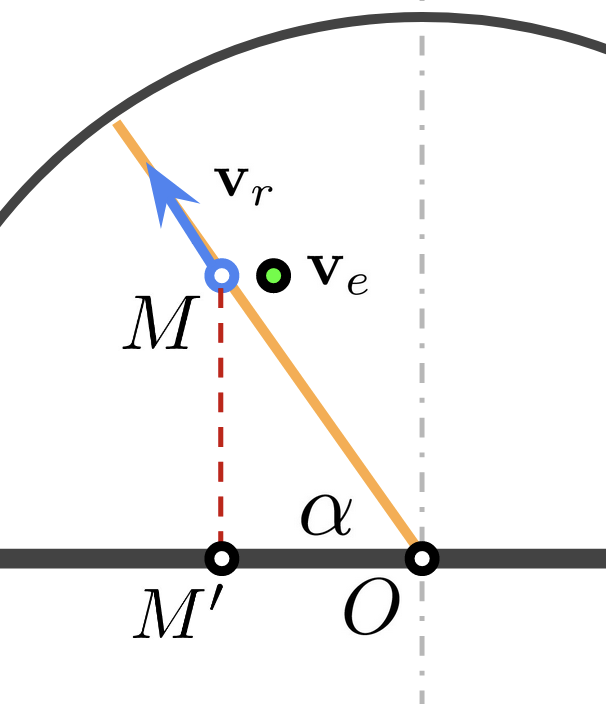
\includegraphics[width=0.3\textwidth]{images/test_1/fig_3.png}
    \caption{Швидкості}
    \label{fig:3}
\end{figure}

Відносна швидкість $\mathbf{v}_r$ направлена вздовж $OM$ і по модулю дорівнює $v_r=\dot{s}$. Переносна швидкість $\mathbf{v}_e$ направлена перпендикулярно площині малюнку і дорівнює $v_e=MM' \cdot \omega$ по модулю. З геометрії $MM' = s(t)\sin\alpha$. Таким чином, $v_e=\omega(t)s(t)\sin\alpha$. Абсолютна швидкість $\mathbf{v}=\mathbf{v}_e+\mathbf{v}_r$ і оскільки вектори $\mathbf{v}_e$ та $\mathbf{v}_r$ перпендикулярні, модуль:
\[
v^2 = v_e^2 + v_r^2 = \dot{s}^2 + \omega^2s^2\sin^2\alpha = \dot{s}^2 + \dot{\varphi}^2s^2\sin^2\alpha
\]
Далі розрахунки такі самі, як в \textit{Способі I}. 

Перейдемо до розрахунку прискорення. Прискорення:
\[
\mathbf{a} = \mathbf{a}_r + \mathbf{a}_e + \mathbf{a}_K
\]
де $\mathbf{a}_K$ -- прискорення Коріоліса. 

Ці компоненти зображені на рис. \ref{fig:4} ($\mathbf{a}_e=\mathbf{a}_n+\mathbf{a}_{\tau}$).

\begin{figure}[H]
    \centering
    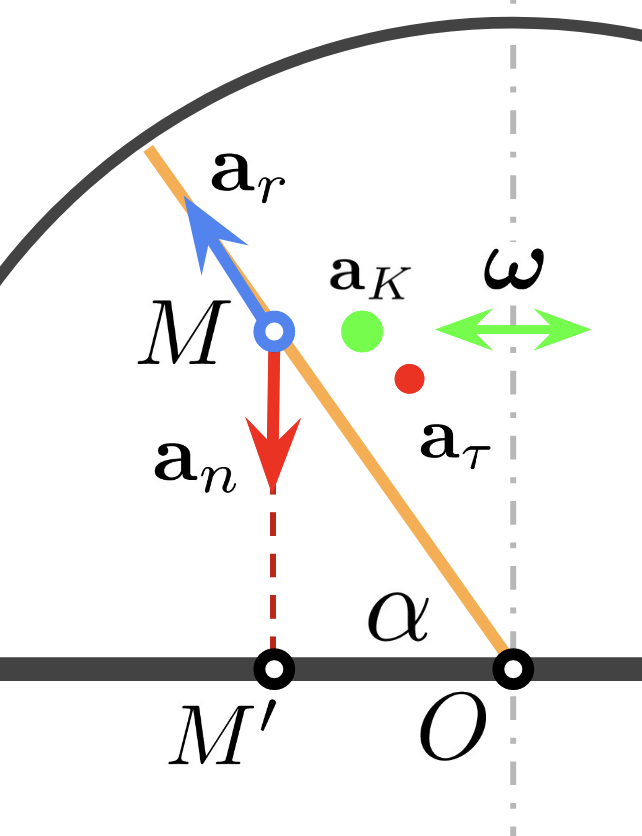
\includegraphics[width=0.3\textwidth]{images/test_1/fig_4.png}
    \caption{Прискорення. Напрям кутової швидкості $\boldsymbol{\omega}$ ми не визначаємо, оскільки це непринципово (а помилитися можна :)). $\mathbf{a}_K$ та $\mathbf{a}_{\tau}$ направлені перпендикулярно площині малюнку.}
    \label{fig:4}
\end{figure}

Розглянемо кожен доданок окремо. Відносне прискорення по модулю дорівнює $a_r=\ddot{s}$ і направлено вздовж $OM$. 

Переносне прискорення дорівнює сумі доцентрового прискорення і тангенсального по колу. Доцентрове прискорення направлено вздовж $MM'$. Модуль доцентрового прискорення дорівнює $a_n=\omega^2\cdot MM' = \omega^2s \sin\alpha$, а тангенсального $a_{\tau}=\varepsilon \cdot MM' = \ddot{\varphi}s \sin\alpha$ і направлено перпендикулярно площині малюнку. 

Нарешті, прискорення Коріоліса, за означенням, $\mathbf{a}_K = 2[\boldsymbol{\omega} \times \mathbf{v}_r]$. Вектори $\boldsymbol{\omega}$ та $\mathbf{v}_r$ знаходяться в одній площині, тому вектор направлений перпендикулярно площині малюнку. Оскільки кут між векторами $\alpha$, то модуль цього прискорення $a_K = 2\omega v_r \sin\alpha = 2\dot{\varphi}\dot{s}\sin\alpha$.

Тепер знайдемо векторну суму, спроектувавши все на вісі $Ox',Oy',Oz'$ (орієнтація на рис. \ref{fig:2}). 
По горизонтальній вісі маємо
\[
a_x = -a_r \cos\alpha = -\ddot{s}\cos\alpha
\]
По вертикальній вісі:
\[
a_y = a_r \sin\alpha - a_n = \ddot{s}\sin\alpha - \dot{\varphi}^2s \sin \alpha = (\ddot{s} - \dot{\varphi}^2 s)\sin\alpha
\]
А перпендикулярно площині малюнку (можна перевірити, що $a_K$ та $a_{\tau}$ сонаправлені для будь-якої орієнтації $\boldsymbol{\omega}$):
\[
|a_z| = a_\tau + a_K = 2\dot{\varphi}\dot{s}\sin\alpha + \ddot{\varphi} s \sin\alpha =  (2\dot{\varphi}\dot{s}+\ddot{\varphi}s)\sin\alpha
\]
Таким чином, модуль:
\[
a^2 = ((\ddot{s}-\dot{\varphi}^2s)^2 + (2\dot{\varphi}\dot{s}+\ddot{\varphi}s)^2)\sin^2\alpha + \ddot{s}^2\cos^2\alpha
\]
Підставляємо числа. $\ddot{s}(t_1)=6t=1.2 \, \frac{\text{m}}{\text{s}^2}$, $s(t_1)=2.8 \, \text{m}$, $\dot{\varphi}(t_1)=4\, \frac{\text{rad}}{\text{s}}$. Тому:
\[
a^2 = 1534.2 \implies a \approx 39.2 \, \frac{\text{m}}{\text{s}^2}
\]

\end{document}

